%clase del documento
\documentclass[a4paper,12pt]{article}

%paquete de idioma y codificación de caracteres
\usepackage[spanish]{babel}
\usepackage[utf8]{inputenc}


% soporte gráfico
\usepackage{graphicx}
\graphicspath{ {images/} }

%datos del documento
\title{Especificación Gráfica de Procesos de Recuperación de Datos en LUCA
}
\author{Ignacio Agüero Salcines}


\begin{document}
	
	\maketitle
	
	\newpage

	{\Large Contexto y  Motivación del proyecto}\\

	Las empresas actuales utilizan ya no un único sistema de información que de
	soporte a sus procesos de trabajo, sino un  ecosistema de sistemas información
	que dan soporte a diferentes procesos de negocio ejecutados dentro de dicha
	organización. Como consecuencia de esta nueva situación, cuando un usuario
	quiere obtener una información concreta cuyos datos residen en varios de estos
	sistemas, necesita acceder a cada uno de estos sistemas, extraer de cada
	sistema la información que precisa, filtrarla y unificarla para finalmente
	obtener los datos requeridos.\\
	
	Por ejemplo, una tienda de electrodomésticos podría tener sistemas informáticos
	diferentes para el departamento de atención al cliente, para el departamento
	técnico de postventa y para el departamento de compras y adquisiciones.
	Por tanto, para conocer el estado actual de una reparación, podríamos necesitar:
	(1) acceder al primer sistema para obtener el identificador de la incidencia y
	en qué fase de su gestión se encuentra; (2) comprobado que la incidencia está
	actualmente en reparación, recuperaríamos otro sistema el estado detallado de
	la reparación, comprobando que está a la espera de una pieza; y (3) finalmente
	accederíamos al sistema de compra y adquisiciones para comprobar cuando está
	prevista la entrega de dicha pieza. Los sistemas de almacenamiento de la
	información puede ser diversos, incluyendo desde un servicio web, una base de
	datos relacional, un repositorio de ficheros accesible vía FTP o una base de
	datos NoSQL.\\
 
	
	Con el objeto de facilitar este proceso de recuperación de información
	almecenada en sistemas y fuentes de datos hetereogéneas, dentro de la empresa
	CIC, se está desarrollando una aplicación denominada LUCA. Para
	facilitar este proceso de recuperación de información, LUCA proporciona un
	lenguaje común para todas las fuentes de datos a unificar, permitiendo al
	usuario abstraerse de los detalles de cada fuente.
	
	Actualmente LUCA proporciona mecanismos o abstracciones para permitir al
	usuario recuperar de manera uniforme información de diferentes fuentes de datos.
	Utilizando el ejemplo anterior, LUCA actualmente propociona mecanismos para
	recuperar información, de la misma forma y mediante las mismas primitivas, de
	los tres sistemas previamente descritos, aunque sus sistemas de almacenamiento
	sean radicalmente diferentes.
	
	No obstante, LUCA actualmente sólo es capaz recuperar información de una única
	fuente de datos a la vez. Por tanto, cuando es necesario combinar
	información procedente de distintas fuentes, tal como ocurre en el ejemplo
	descrito, el propio usuario es el que debe realizar dicho
	proceso de composición, ejecutando cada consulta a mano, y utilizando las
	salidas de cada una de ellas como las entradas de las siguientes.
	
	
		\begin{center}
		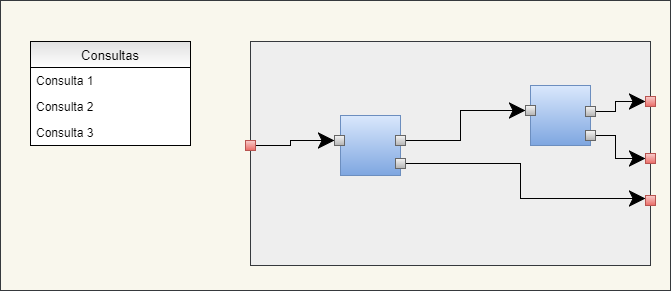
\includegraphics[width=12cm]{images/ejemploDiagrama}\\
	\end{center}
	
	
	El objetivo de este proyecto es facilitar dicho proceso de composición al
	usuario mediante el desarrollo de un mecanismo gráfico para la especificación
	de estos procesos de composición de consultas.
	
	Dado que la empresa solicita que este editor gráfico sea utilizable vía web,
	se desarrollará utilizando la librería gráfica Javscript Go.JS y el framework
	Vaadin.
	
	\newpage
	{\Large Arquitectura y/o tecnologías del proyecto}\\
	
	El componente genérico se compone de dos soportes principales, uno mediante la herramienta javascript GO.JS, el cuál se encargara de visualizar gráficamente los datos (aunque también contiene una lógica interna propia a desarrollar), y otro soporte lógico encargado presentar el patrón MVP (modelo vista presentador), que interactuará con la herramienta gráfica.\\
	
	\begin{center}
		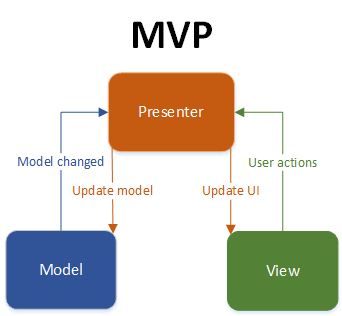
\includegraphics{images/mvp}\\
	\end{center}
	
	
	Este ensamblado de herramientas se realizará usando Vaadin, el cuál, mediante un fichero conector escrito en javascript, se encargará de realizar las comunicaciones entre la parte lógica y la parte gráfica.\\
	
	
	\begin{center}
		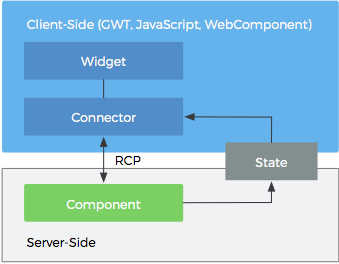
\includegraphics{images/schema}\\
	\end{center}
	

	
\end{document}